\subsubsection{Description}\label{subsec:precharge}

\begin{figure}[H]
	\centering
	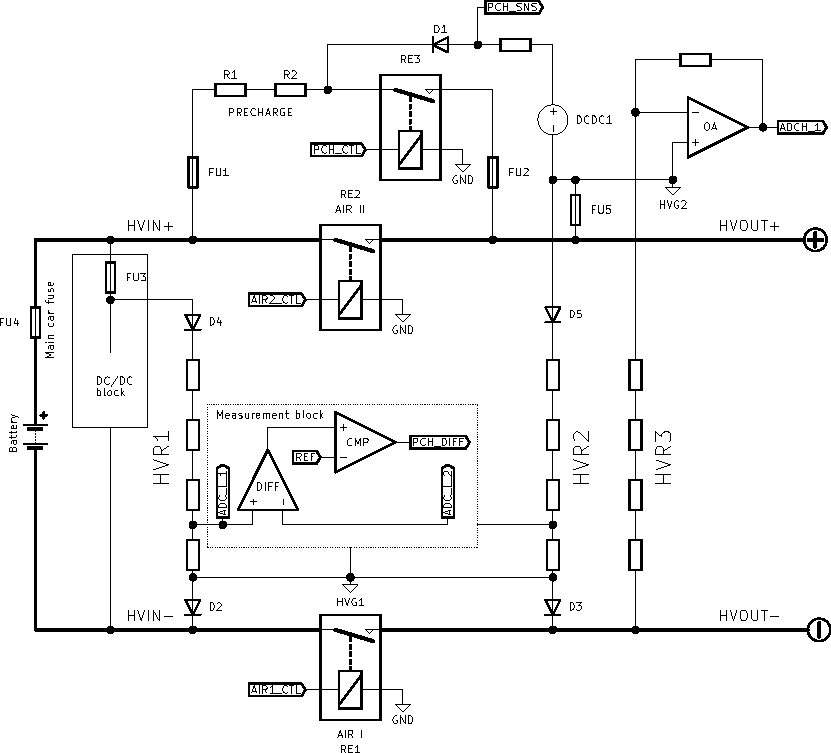
\includegraphics[width=\textwidth,clip]{./img/ECUA_AIRS.pdf}
	\caption{TS pre-charge circuit and switching schematic.}
	\label{fig:precharge_sch}
\end{figure}

Principial block schematic of the TS switching circuit (including pre-charge) is in the \ref{fig:precharge_sch}. Pre-charge circuit is part of and controlled by \gls{ecua}. Pre-charge circuit is comprised of a relay RE$_3$ and two series connected power resistors R$_1$ and R$_2$. The pre-charge circuit is fused by a fast blow 2 A 500 V rated fuse (\ref{app:precharge_fuse_datasheet}). 

Both resistors are located on a heat-sink, that is shared with the DC/DC converters, mentioned in \ref{subsec:glvs_dcdc} of this document. The task of the heat-sink is to enhance the power overload capacity of the pre-charge resistors during the initial overload during the beginning of the charging curve, shown in \ref{fig:precharge_voltage_time}.

\begin{figure}
	\begin{tikzpicture}
		\begin{axis}[
			use units,
			x unit=s,
			y unit=V,
			xlabel=time,
			ylabel=volatge,
			width=0.9\textwidth,
			height=0.5\textwidth,
			grid=major,
			xmin=0,
			ymin=0,
			xmax=10
			]
		\addplot[red, smooth] table[
			x=time,
			y=voltage,
			col sep=comma
			] {./data/TS_precharge.csv};
		\end{axis}
		\end{tikzpicture}
		\caption{Pre-charge voltage in time.}
	\label{fig:precharge_voltage_time}
\end{figure}

The formula describing \ref{fig:precharge_voltage_time} is:

\begin{equation}
	V_{c}=V_{s}*(1-e^{(\frac{-t}{R*C})})
	\label{eq:precharge_voltage}
\end{equation}

\begin{figure}
	\begin{tikzpicture}
	\begin{axis}[
	use units,
	x unit=s,
	y unit=A,
	xlabel=time,
	ylabel=current,
	width=0.9\textwidth,
	height=0.5\textwidth,
	grid=major,
	xmin=0,
	ymin=0,
	xmax=10
	]
	\addplot[red, smooth] table[
	x=time,
	y=current,
	col sep=comma
	] {./data/TS_precharge.csv}; 
	\end{axis}
	\end{tikzpicture}
	\caption{Precharge current in time.}
	\label{fig:precharge_current_time}
\end{figure}

The formula describing \ref{fig:precharge_current_time} is:

\begin{equation}
	I=\frac{V_{c}-V_{s}}{R}	
	\label{eq:precharge_current}
\end{equation}


Both wirewound power resistors, ARCOL HS25 series, have 250 $\Omega$, 25 W continuous rating, (\ref{app:precharge_resistors}).

All three TS relays RE$_1$ to RE$_3$ coils are powered directly from the \gls{sdc} end.

After the \gls{sdc} circuit is complete and closed (voltage present at \gls{sdc} END), the pre-charge sequence is begun by closing AIR I (RE$_1$). Then a pre-charge relay RE$_3$ is closed. Voltage both on the \gls{acp} and output side is monitored using the measurement block, through the $HVR_1$ and HVR$_2$ resistor dividers. After the voltage difference is low enough (determined by \gls{ecua} software), AIR II (RE$_2$) is closed, RE$_3$ can be released.

Safety of the \gls{air} switching and pre-charging is done by the \gls{ecua} firmware, that evaluates all possible circuit states. Voltages are measured on the \gls{acp} and \gls{acp} output sides using the measurement block, AIR physical states are observed using the auxiliary contacts and the pre-charge relay physical contact state is observed using the principle in the \ref{fig:precharge_sch}, via the diode D$_1$. The PCH\_SNS signal is pulled low whenever the pre-charge relay RE$_3$ contact is closed.

Several safety precautions are implemented, on top of the Rules. First of such implemented protections is HW non-programmable voltage difference sensing across the pre-charge relay or AIR II respectively. This is done using the two voltage measurement dividers HVR$_1$ and HVR$_2$. There is a differential amplifier and comparator, that prevents closing both AIR relays in case of high voltage difference across the AIR II. 

Diodes D$_2$ and D$_3$ serve to block current flow to the output in case of AIR I is open. This specific topology was chosen to be able to measure the difference voltage across the AIR II utilizing only analog non-programmable circuitry.

Second precaution is a \gls{hv} circuit limiting the maximum pre-charge relay closed time, and assuring a minimum off time for the pre-charge resistor to cool off. This circuit is a non-programmable one, realized using a discrete logic. \phantomsection\label{precharge_arc_breaking}

Additional precision \gls{acp} voltage measurement is taken using the HVR$_3$ sense divider, as this measurement is not influenced by the forward voltage drops of diodes D$_2$ to D$_5$. This measurement together with the measured \gls{acp} current serves to calculate power drawn from the \gls{acp}. This measurement is then presented on the \gls{can} bus for other car \glspl{ecu}, for example to estimate the SOC, instantaneous power, etc.  

The TS voltage sensing dividers HVR$_1$, HVR$_2$ and HVR$_3$ are realized with a high voltage 3500 V rated resistors from Vishay, HVR$_{37}$ series (\ref{app:hvr37_datasheet}). All dividers use 10 M$\Omega$ resistors as the top side of the divider. All diodes D$_1$ to D$_5$ are SM4007 (DATASHEET) or equivalent type, 1000 V rated. The blocking voltage is therefore sufficient to safely withstand the maximum \gls{acp} voltage of 408 V.

\paragraph{Pre-charge safety on \gls{ecua}}
Except from what rules require we implemented several safety precautions. In case, that \gls{sdc} error does not occur and driver pushed TS ON button following safety precautions are taken to prevent switching AIR in case of problem that has not yet been detected.

First one is completely non-programmable protection against switching voltage difference by \gls{air}. It uses voltage measurement and then comparators and logic to disable \gls{mcu} decision in case of SW error.
Second one is measuring all states and voltages by \gls{mcu} on \gls{ecua} which can determinate error before non-programmable protection would have to act.

Third (time-out) protection is used when everything seems to be OK, but the charging is too slow – caused by too high pre-charge resistance (any of pre-charge resistors fails), or some leakage of charge in capacitor or any other possible error occurs. If voltage difference is not equaled in time less them 2 seconds, the \gls{ecua} stops pre-charge and waits 5 seconds before trying again. (In order to not overpower resistors.) If number of attempts to pre-charge is in this state higher then 8, something is clearly wrong and \gls{ecua} opens \gls{sdc} and indicates error. Sending message about error and sets car into not-ready state.

\subsubsection{Wiring, cables, current calculations, connectors}
%Describe wiring, show schematics, describe connectors and cables used and show useful data regarding the wiring.

%\item Give a plot “Percentage of Maximum Voltage” vs. time
%\item Give a plot Current vs. time 
%\item For each plot, give the basic formula describing the plots
There is no connectors nor cables it is realised on \gls{pcb} in \gls{ecua}. 

%Additionally, fill out the tables:

\begin{table}[H]
	\centering
	\caption{General data of the pre-charge resistor}
	\begin{tabu}{|X|X|}
		\hline
		Resistor Type: & Wirewound \\
		\hline

		Resistance: & 250 $\Omega$ in 2s configuration (500 $\Omega$ in total) \\
		\hline
		Continuous power rating: & 25 W per resistor (50 W  in total)\\
		\hline
		Overload power rating (1 sec): & 250 W per resistor (500 W in total) \\
		\hline
		Overload power rating (5 sec): & 125 W per resistor (250 W in total) \\
		\hline
		Overload power rating (15 sec): & not specified \\
		\hline
		Voltage rating: & 680 V$_{AC}$\\
		\hline
		Cross-sectional area of the wire used: & 0.195 mm$^2$\\
		\hline
	\end{tabu}%
	\label{tab:precharge-general}%
\end{table}%

\ref{app:precharge_resistors}

\ref{app:precharge_resistors_overload}


\begin{table}[H]
	\centering
	\caption{General data of the pre-charge relay}
	\begin{tabu}{|X|X|}
		\hline
		Relay Type: & Meder  LI24-1A85\\
		\hline
		Contact arrangement: &  SPST-NO \\
		\hline
		Continuous DC current:  & 2.5 A\\
		\hline
		Voltage rating  & 1000 V\\
		\hline
		Nominal Coil Voltage: & 24 V \\
		\hline
		Cross-sectional area of the wire used: & 0.195 mm$^2$ \\
		\hline
	\end{tabu}%
	\label{tab:precharge-relay}%
\end{table}%

\ref{app:precharge_relay_datasheet}

\subsubsection{Position in car}
%Provide CAD-renderings showing all relevant parts. Mark the parts in the rendering, if necessary.

\begin{figure}[H]
	\centering
	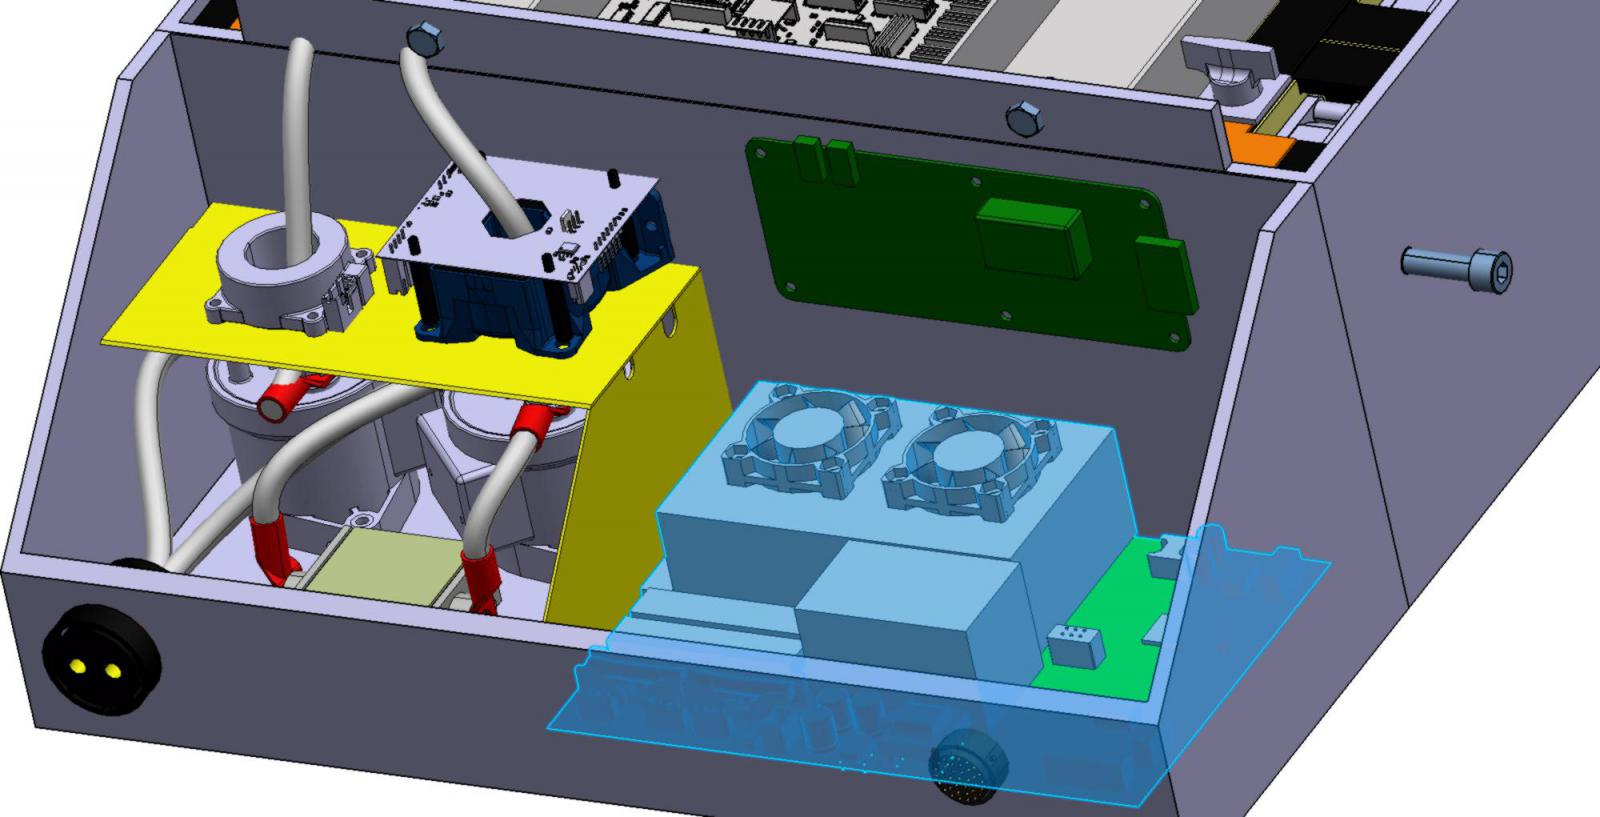
\includegraphics[width=\textwidth]{./img/ECUA_POSITION.jpg}
	\caption{ECUA position.}
	\label{fig:ECUA}
\end{figure}